% Options for packages loaded elsewhere
\PassOptionsToPackage{unicode}{hyperref}
\PassOptionsToPackage{hyphens}{url}
%
\documentclass[
]{article}
\usepackage{lmodern}
\usepackage{amssymb,amsmath}
\usepackage{ifxetex,ifluatex}
\ifnum 0\ifxetex 1\fi\ifluatex 1\fi=0 % if pdftex
  \usepackage[T1]{fontenc}
  \usepackage[utf8]{inputenc}
  \usepackage{textcomp} % provide euro and other symbols
\else % if luatex or xetex
  \usepackage{unicode-math}
  \defaultfontfeatures{Scale=MatchLowercase}
  \defaultfontfeatures[\rmfamily]{Ligatures=TeX,Scale=1}
\fi
% Use upquote if available, for straight quotes in verbatim environments
\IfFileExists{upquote.sty}{\usepackage{upquote}}{}
\IfFileExists{microtype.sty}{% use microtype if available
  \usepackage[]{microtype}
  \UseMicrotypeSet[protrusion]{basicmath} % disable protrusion for tt fonts
}{}
\makeatletter
\@ifundefined{KOMAClassName}{% if non-KOMA class
  \IfFileExists{parskip.sty}{%
    \usepackage{parskip}
  }{% else
    \setlength{\parindent}{0pt}
    \setlength{\parskip}{6pt plus 2pt minus 1pt}}
}{% if KOMA class
  \KOMAoptions{parskip=half}}
\makeatother
\usepackage{xcolor}
\IfFileExists{xurl.sty}{\usepackage{xurl}}{} % add URL line breaks if available
\IfFileExists{bookmark.sty}{\usepackage{bookmark}}{\usepackage{hyperref}}
\hypersetup{
  pdftitle={English Premier League Match Predictor},
  pdfauthor={Omotoyosi Taiwo},
  hidelinks,
  pdfcreator={LaTeX via pandoc}}
\urlstyle{same} % disable monospaced font for URLs
\usepackage[margin=1in]{geometry}
\usepackage{color}
\usepackage{fancyvrb}
\newcommand{\VerbBar}{|}
\newcommand{\VERB}{\Verb[commandchars=\\\{\}]}
\DefineVerbatimEnvironment{Highlighting}{Verbatim}{commandchars=\\\{\}}
% Add ',fontsize=\small' for more characters per line
\usepackage{framed}
\definecolor{shadecolor}{RGB}{248,248,248}
\newenvironment{Shaded}{\begin{snugshade}}{\end{snugshade}}
\newcommand{\AlertTok}[1]{\textcolor[rgb]{0.94,0.16,0.16}{#1}}
\newcommand{\AnnotationTok}[1]{\textcolor[rgb]{0.56,0.35,0.01}{\textbf{\textit{#1}}}}
\newcommand{\AttributeTok}[1]{\textcolor[rgb]{0.77,0.63,0.00}{#1}}
\newcommand{\BaseNTok}[1]{\textcolor[rgb]{0.00,0.00,0.81}{#1}}
\newcommand{\BuiltInTok}[1]{#1}
\newcommand{\CharTok}[1]{\textcolor[rgb]{0.31,0.60,0.02}{#1}}
\newcommand{\CommentTok}[1]{\textcolor[rgb]{0.56,0.35,0.01}{\textit{#1}}}
\newcommand{\CommentVarTok}[1]{\textcolor[rgb]{0.56,0.35,0.01}{\textbf{\textit{#1}}}}
\newcommand{\ConstantTok}[1]{\textcolor[rgb]{0.00,0.00,0.00}{#1}}
\newcommand{\ControlFlowTok}[1]{\textcolor[rgb]{0.13,0.29,0.53}{\textbf{#1}}}
\newcommand{\DataTypeTok}[1]{\textcolor[rgb]{0.13,0.29,0.53}{#1}}
\newcommand{\DecValTok}[1]{\textcolor[rgb]{0.00,0.00,0.81}{#1}}
\newcommand{\DocumentationTok}[1]{\textcolor[rgb]{0.56,0.35,0.01}{\textbf{\textit{#1}}}}
\newcommand{\ErrorTok}[1]{\textcolor[rgb]{0.64,0.00,0.00}{\textbf{#1}}}
\newcommand{\ExtensionTok}[1]{#1}
\newcommand{\FloatTok}[1]{\textcolor[rgb]{0.00,0.00,0.81}{#1}}
\newcommand{\FunctionTok}[1]{\textcolor[rgb]{0.00,0.00,0.00}{#1}}
\newcommand{\ImportTok}[1]{#1}
\newcommand{\InformationTok}[1]{\textcolor[rgb]{0.56,0.35,0.01}{\textbf{\textit{#1}}}}
\newcommand{\KeywordTok}[1]{\textcolor[rgb]{0.13,0.29,0.53}{\textbf{#1}}}
\newcommand{\NormalTok}[1]{#1}
\newcommand{\OperatorTok}[1]{\textcolor[rgb]{0.81,0.36,0.00}{\textbf{#1}}}
\newcommand{\OtherTok}[1]{\textcolor[rgb]{0.56,0.35,0.01}{#1}}
\newcommand{\PreprocessorTok}[1]{\textcolor[rgb]{0.56,0.35,0.01}{\textit{#1}}}
\newcommand{\RegionMarkerTok}[1]{#1}
\newcommand{\SpecialCharTok}[1]{\textcolor[rgb]{0.00,0.00,0.00}{#1}}
\newcommand{\SpecialStringTok}[1]{\textcolor[rgb]{0.31,0.60,0.02}{#1}}
\newcommand{\StringTok}[1]{\textcolor[rgb]{0.31,0.60,0.02}{#1}}
\newcommand{\VariableTok}[1]{\textcolor[rgb]{0.00,0.00,0.00}{#1}}
\newcommand{\VerbatimStringTok}[1]{\textcolor[rgb]{0.31,0.60,0.02}{#1}}
\newcommand{\WarningTok}[1]{\textcolor[rgb]{0.56,0.35,0.01}{\textbf{\textit{#1}}}}
\usepackage{graphicx,grffile}
\makeatletter
\def\maxwidth{\ifdim\Gin@nat@width>\linewidth\linewidth\else\Gin@nat@width\fi}
\def\maxheight{\ifdim\Gin@nat@height>\textheight\textheight\else\Gin@nat@height\fi}
\makeatother
% Scale images if necessary, so that they will not overflow the page
% margins by default, and it is still possible to overwrite the defaults
% using explicit options in \includegraphics[width, height, ...]{}
\setkeys{Gin}{width=\maxwidth,height=\maxheight,keepaspectratio}
% Set default figure placement to htbp
\makeatletter
\def\fps@figure{htbp}
\makeatother
\setlength{\emergencystretch}{3em} % prevent overfull lines
\providecommand{\tightlist}{%
  \setlength{\itemsep}{0pt}\setlength{\parskip}{0pt}}
\setcounter{secnumdepth}{-\maxdimen} % remove section numbering

\title{English Premier League Match Predictor}
\author{Omotoyosi Taiwo}
\date{}

\begin{document}
\maketitle

\hypertarget{introduction}{%
\subsection{Introduction}\label{introduction}}

Football Matches are notoriously hard to predict due to the random and
low scoring nature of the games. One of the prevailing nuggets of wisdom
however, is that home teams win more on average, and this has been
statistically backed up. In recent years, more advanced metrics have
been proposed to account for variance in playing styles and team
performances. An example is xG (Expected Goals) this is a measure the
possible goals teams should have scored based on shot location, however
even that does not account for factors like defence engagement, the time
the shot was attempted, and the current scoreline all which
hypothetically affect players.

These factors and many have made soccer results really difficult to
predict. Betting companies develop advanced algortithms to generate true
odds for football matches even though they adjust these odds so that
they always turn a profit.

The idea behind this project is to use the closing betting data, team
form (using rolling averages of n previous games for various performance
metrics) and 538 metrics including expected goals, team reputation
(SPI), and projected scores to improve prediction.

The data I used for this project was downloaded from football-data.co.uk
and fivethirtyeight.com

\begin{quote}
Note
\end{quote}

Because 538 metrics only go back to the beginning of the 16/17 season,
the models I generated were finicky and I decided to use only betting
data and team form for various performance metrics like shots on target,
shots allowed, corners, fouls, yellow cards, and red cards

\hypertarget{preparing-the-data}{%
\subsection{Preparing the Data}\label{preparing-the-data}}

I use R data.table, because I love how blazing fast data.tables are and
it's one-liner approach to data manipulation, although it is quite
unneccesary for the size of data involved in this project, however I
plan to include other leagues in the future, and I can see the data
getting big (Big data?) very quickly.

\begin{Shaded}
\begin{Highlighting}[]
\CommentTok{#All functions}
\CommentTok{#Takes confusion_matrix object and plots it with important metrics}
\NormalTok{plot_confusion_matrix =}\StringTok{ }\ControlFlowTok{function}\NormalTok{(cm )\{}
  \KeywordTok{autoplot}\NormalTok{(cm, }\DataTypeTok{type =} \StringTok{"heatmap"}\NormalTok{)}\OperatorTok{+}
\StringTok{  }\KeywordTok{scale_fill_gradient}\NormalTok{(}\DataTypeTok{low=}\StringTok{"#D6EAF8"}\NormalTok{,}\DataTypeTok{high =} \StringTok{"#2E86C1"}\NormalTok{)}\OperatorTok{+}
\StringTok{  }\KeywordTok{ggtitle}\NormalTok{(}\KeywordTok{paste0}\NormalTok{(}\StringTok{"Accuracy = "}\NormalTok{, }\KeywordTok{format}\NormalTok{(}\KeywordTok{round}\NormalTok{(}\KeywordTok{summary}\NormalTok{(cm)[[}\StringTok{".estimate"}\NormalTok{]][}\DecValTok{1}\NormalTok{], }\DecValTok{2}\NormalTok{), }\DataTypeTok{nsmall =} \DecValTok{2}\NormalTok{),}
          \StringTok{"         Sensitivity = "}\NormalTok{, }\KeywordTok{format}\NormalTok{(}\KeywordTok{round}\NormalTok{(}\KeywordTok{summary}\NormalTok{(cm)[[}\StringTok{".estimate"}\NormalTok{]][}\DecValTok{3}\NormalTok{], }\DecValTok{2}\NormalTok{), }\DataTypeTok{nsmall =} \DecValTok{2}\NormalTok{),}
          \StringTok{"         Specificity = "}\NormalTok{, }\KeywordTok{format}\NormalTok{(}\KeywordTok{round}\NormalTok{(}\KeywordTok{summary}\NormalTok{(cm)[[}\StringTok{".estimate"}\NormalTok{]][}\DecValTok{4}\NormalTok{], }\DecValTok{2}\NormalTok{), }\DataTypeTok{nsmall =} \DecValTok{2}\NormalTok{))) }\OperatorTok{+}
\StringTok{  }\KeywordTok{theme}\NormalTok{(}\DataTypeTok{plot.title =} \KeywordTok{element_text}\NormalTok{(}\DataTypeTok{hjust =} \FloatTok{0.5}\NormalTok{))}
\NormalTok{  \} }

\CommentTok{##Custom function - Find the rolling mean of previous n elements}
\NormalTok{shift_froll =}\StringTok{ }\ControlFlowTok{function}\NormalTok{(x, n)\{}\KeywordTok{shift}\NormalTok{(}\KeywordTok{frollmean}\NormalTok{(x, }\DataTypeTok{n=}\NormalTok{ n))\}}
\end{Highlighting}
\end{Shaded}

Read data for the past 20 seasons, this is how far back I could find
gambling data for matches

\begin{Shaded}
\begin{Highlighting}[]
\CommentTok{# Read Match Stats and Betting data}
\ControlFlowTok{for}\NormalTok{ (year }\ControlFlowTok{in} \KeywordTok{c}\NormalTok{(}\DecValTok{0}\OperatorTok{:}\DecValTok{19}\NormalTok{))\{}
\NormalTok{  thisYear =}\StringTok{ }\KeywordTok{print}\NormalTok{(}\KeywordTok{sprintf}\NormalTok{(}\StringTok{"%02d"}\NormalTok{, year))}
\NormalTok{  nextYear =}\StringTok{ }\KeywordTok{print}\NormalTok{(}\KeywordTok{sprintf}\NormalTok{(}\StringTok{"%02d"}\NormalTok{, year}\OperatorTok{+}\DecValTok{1}\NormalTok{))}
  \KeywordTok{assign}\NormalTok{(}\KeywordTok{paste0}\NormalTok{(}\StringTok{"EPL"}\NormalTok{,thisYear,nextYear), }\KeywordTok{fread}\NormalTok{(}\KeywordTok{paste0}\NormalTok{(}\StringTok{"season-"}\NormalTok{,thisYear,nextYear,}\StringTok{"_csv.csv"}\NormalTok{)))}
\NormalTok{\}}
\KeywordTok{setnames}\NormalTok{(EPL1920,}\KeywordTok{c}\NormalTok{(}\StringTok{"AvgA"}\NormalTok{,}\StringTok{"AvgH"}\NormalTok{,}\StringTok{"AvgD"}\NormalTok{), }\KeywordTok{c}\NormalTok{(}\StringTok{"BbAvA"}\NormalTok{,}\StringTok{"BbAvH"}\NormalTok{,}\StringTok{"BbAvD"}\NormalTok{))}\CommentTok{#Fix closing betting averages column name changes from the 19/20 season dataset}

\NormalTok{modelData =}\StringTok{ }\OtherTok{NULL}
\CommentTok{# Seperate Modelling Data that doesn't need to be aggregated}
\NormalTok{modelCols =}\StringTok{ }\KeywordTok{c}\NormalTok{(}\StringTok{"HomeTeam"}\NormalTok{,}\StringTok{"AwayTeam"}\NormalTok{,}\StringTok{"FTR"}\NormalTok{,}\StringTok{"BbAvH"}\NormalTok{,}\StringTok{"BbAvD"}\NormalTok{,}\StringTok{"BbAvA"}\NormalTok{)}
\NormalTok{relevantColumns =}\StringTok{ }\KeywordTok{c}\NormalTok{(}\StringTok{"HomeTeam"}\NormalTok{,}\StringTok{"AwayTeam"}\NormalTok{,}\StringTok{"FTHG"}\NormalTok{,}\StringTok{"FTAG"}\NormalTok{,}\StringTok{"HTHG"}\NormalTok{,}\StringTok{"HTAG"}\NormalTok{,}\StringTok{"HS"}\NormalTok{,}\StringTok{"AS"}\NormalTok{,}\StringTok{"HST"}\NormalTok{,}\StringTok{"AST"}\NormalTok{,}\StringTok{"HF"}\NormalTok{,}\StringTok{"AF"}\NormalTok{,}\StringTok{"HC"}\NormalTok{,}\StringTok{"AC"}\NormalTok{,}\StringTok{"HY"}\NormalTok{,}\StringTok{"AY"}\NormalTok{,}\StringTok{"HR"}\NormalTok{,}\StringTok{"AR"}\NormalTok{)}
\NormalTok{allSeasons =}\StringTok{ }\KeywordTok{vector}\NormalTok{(}\DataTypeTok{mode=}\StringTok{"list"}\NormalTok{, }\DataTypeTok{length =} \DecValTok{20}\NormalTok{)}
\NormalTok{meltedDataList =}\StringTok{ }\KeywordTok{list}\NormalTok{()}
\ControlFlowTok{for}\NormalTok{ (year }\ControlFlowTok{in} \KeywordTok{c}\NormalTok{(}\DecValTok{0}\OperatorTok{:}\DecValTok{19}\NormalTok{))\{}
\NormalTok{  thisYear =}\StringTok{ }\KeywordTok{print}\NormalTok{(}\KeywordTok{sprintf}\NormalTok{(}\StringTok{"%02d"}\NormalTok{, year))}
\NormalTok{  nextYear =}\StringTok{ }\KeywordTok{print}\NormalTok{(}\KeywordTok{sprintf}\NormalTok{(}\StringTok{"%02d"}\NormalTok{, year}\OperatorTok{+}\DecValTok{1}\NormalTok{))}
  \KeywordTok{assign}\NormalTok{(}\KeywordTok{paste0}\NormalTok{(}\StringTok{"EPL"}\NormalTok{,thisYear,nextYear,}\StringTok{"Mod"}\NormalTok{), }\KeywordTok{get}\NormalTok{(}\KeywordTok{paste0}\NormalTok{(}\StringTok{"EPL"}\NormalTok{,thisYear,nextYear))[,..modelCols] )}
\NormalTok{  modelData =}\StringTok{ }\KeywordTok{rbind}\NormalTok{(modelData, }\KeywordTok{get}\NormalTok{(}\KeywordTok{paste0}\NormalTok{(}\StringTok{"EPL"}\NormalTok{,thisYear,nextYear,}\StringTok{"Mod"}\NormalTok{)))}
  \KeywordTok{assign}\NormalTok{(}\KeywordTok{paste0}\NormalTok{(}\StringTok{"EPL"}\NormalTok{,thisYear,nextYear), }\KeywordTok{get}\NormalTok{(}\KeywordTok{paste0}\NormalTok{(}\StringTok{"EPL"}\NormalTok{,thisYear,nextYear))[,..relevantColumns])}
\NormalTok{  allSeasons[[year}\OperatorTok{+}\DecValTok{1}\NormalTok{]] =}\StringTok{ }\KeywordTok{get}\NormalTok{(}\KeywordTok{paste0}\NormalTok{(}\StringTok{"EPL"}\NormalTok{,thisYear,nextYear))}
\NormalTok{\}}


\CommentTok{#Separate Predictor variables from Aggregators.}
\NormalTok{aggregateEplCols =}\StringTok{ }\KeywordTok{c}\NormalTok{(}\StringTok{"HomeTeam"}\NormalTok{,}\StringTok{"AwayTeam"}\NormalTok{,}\StringTok{"FTHG"}\NormalTok{,}\StringTok{"FTAG"}\NormalTok{,}\StringTok{"HTHG"}\NormalTok{,}\StringTok{"HTAG"}\NormalTok{,}\StringTok{"HS"}\NormalTok{,}\StringTok{"AS"}\NormalTok{,}\StringTok{"HST"}\NormalTok{,}\StringTok{"AST"}\NormalTok{,}\StringTok{"HF"}\NormalTok{,}\StringTok{"AF"}\NormalTok{,}\StringTok{"HC"}\NormalTok{,}\StringTok{"AC"}\NormalTok{,}\StringTok{"HY"}\NormalTok{,}\StringTok{"AY"}\NormalTok{,}\StringTok{"HR"}\NormalTok{,}\StringTok{"AR"}\NormalTok{)}
\NormalTok{seasonMeltMeasureList =}\StringTok{ }\KeywordTok{list}\NormalTok{(}\KeywordTok{c}\NormalTok{(}\StringTok{"HomeTeam"}\NormalTok{, }\StringTok{"AwayTeam"}\NormalTok{), }\KeywordTok{c}\NormalTok{(}\StringTok{"FTHG"}\NormalTok{, }\StringTok{"FTAG"}\NormalTok{), }\KeywordTok{c}\NormalTok{(}\StringTok{"HTHG"}\NormalTok{, }\StringTok{"HTAG"}\NormalTok{), }\KeywordTok{c}\NormalTok{(}\StringTok{"HS"}\NormalTok{, }\StringTok{"AS"}\NormalTok{), }\KeywordTok{c}\NormalTok{(}\StringTok{"HST"}\NormalTok{, }\StringTok{"AST"}\NormalTok{), }\KeywordTok{c}\NormalTok{(}\StringTok{"HF"}\NormalTok{, }\StringTok{"AF"}\NormalTok{), }\KeywordTok{c}\NormalTok{(}\StringTok{"HC"}\NormalTok{, }\StringTok{"AC"}\NormalTok{),}\KeywordTok{c}\NormalTok{(}\StringTok{"HY"}\NormalTok{, }\StringTok{"AY"}\NormalTok{), }\KeywordTok{c}\NormalTok{(}\StringTok{"HR"}\NormalTok{, }\StringTok{"AR"}\NormalTok{))}
\NormalTok{seasonMeltNames =}\StringTok{ }\KeywordTok{c}\NormalTok{(}\StringTok{"Team"}\NormalTok{,}\StringTok{"FTG"}\NormalTok{,}\StringTok{"HTG"}\NormalTok{,}\StringTok{"Shots"}\NormalTok{,}\StringTok{"ST"}\NormalTok{,}\StringTok{"Fouls"}\NormalTok{,}\StringTok{"Corners"}\NormalTok{,}\StringTok{"Yellow"}\NormalTok{,}\StringTok{"Red"}\NormalTok{)}

\CommentTok{#For loop to aggregate each season data}
\ControlFlowTok{for}\NormalTok{(season }\ControlFlowTok{in}\NormalTok{ allSeasons)\{}
  \CommentTok{#Melt to combine home and away results - Note separate running averages in future}
\NormalTok{  season =}\StringTok{ }\KeywordTok{melt}\NormalTok{(season, }\DataTypeTok{measure =}\NormalTok{ seasonMeltMeasureList, }\DataTypeTok{value.name =}\NormalTok{ seasonMeltNames)}
\NormalTok{  meltedDataList[[}\KeywordTok{length}\NormalTok{(meltedDataList)}\OperatorTok{+}\DecValTok{1}\NormalTok{]] <-}\StringTok{ }\NormalTok{season}
\NormalTok{\}}
\NormalTok{allMeltedData =}\StringTok{ }\KeywordTok{rbindlist}\NormalTok{(meltedDataList)}

\CommentTok{#New columns for the rolling Averages}
\NormalTok{rollingAvgColumns =}\StringTok{ }\KeywordTok{paste0}\NormalTok{(}\KeywordTok{c}\NormalTok{(}\StringTok{"FTG"}\NormalTok{,}\StringTok{"HTG"}\NormalTok{,}\StringTok{"Shots"}\NormalTok{,}\StringTok{"ST"}\NormalTok{,}\StringTok{"Fouls"}\NormalTok{,}\StringTok{"Corners"}\NormalTok{,}\StringTok{"Yellow"}\NormalTok{,}\StringTok{"Red"}\NormalTok{),}\StringTok{"rAvg"}\NormalTok{)}
\CommentTok{#bMelted[,variable:= as.factor(variable)]}

\CommentTok{#Rolling Maean and Shift}
\NormalTok{allMeltedData[, (rollingAvgColumns)}\OperatorTok{:}\ErrorTok{=}\StringTok{ }\KeywordTok{lapply}\NormalTok{(.SD, shift_froll,  }\DataTypeTok{n =} \DecValTok{5}\NormalTok{), by =}\StringTok{ }\KeywordTok{c}\NormalTok{(}\StringTok{"Team"}\NormalTok{,}\StringTok{"variable"}\NormalTok{), .SDcols =}\StringTok{  }\KeywordTok{c}\NormalTok{(}\StringTok{"FTG"}\NormalTok{,}\StringTok{"HTG"}\NormalTok{,}\StringTok{"Shots"}\NormalTok{,}\StringTok{"ST"}\NormalTok{,}\StringTok{"Fouls"}\NormalTok{,}\StringTok{"Corners"}\NormalTok{,}\StringTok{"Yellow"}\NormalTok{,}\StringTok{"Red"}\NormalTok{)]}

\CommentTok{#Fill NA values from rolling window and shifting with mean}
\NormalTok{allMeltedData[,}\DecValTok{11}\OperatorTok{:}\DecValTok{18} \OperatorTok{:}\ErrorTok{=}\StringTok{ }\KeywordTok{na.aggregate}\NormalTok{(allMeltedData[,}\DecValTok{11}\OperatorTok{:}\DecValTok{18}\NormalTok{] )]}

\CommentTok{#Modelling Data}
\CommentTok{#--------------}
\CommentTok{#Fold data into Home and Away}
\NormalTok{awayNames =}\StringTok{ }\KeywordTok{names}\NormalTok{(allMeltedData[,}\DecValTok{11}\OperatorTok{:}\DecValTok{18}\NormalTok{])}\CommentTok{#Get table names except variable}
\NormalTok{awayNames =}\StringTok{ }\KeywordTok{paste0}\NormalTok{(awayNames,}\StringTok{"Away"}\NormalTok{)}\CommentTok{#Add away to specify stats}
\NormalTok{allHome =}\StringTok{ }\NormalTok{allMeltedData[variable }\OperatorTok{==}\StringTok{ }\DecValTok{1}\NormalTok{, }\DecValTok{11}\OperatorTok{:}\DecValTok{18}\NormalTok{] }\CommentTok{#Home Stats without variable}
\NormalTok{allAway =}\StringTok{ }\NormalTok{allMeltedData[variable }\OperatorTok{==}\StringTok{ }\DecValTok{2}\NormalTok{, }\DecValTok{11}\OperatorTok{:}\DecValTok{18}\NormalTok{] }\CommentTok{#Away stats without the variable}
\KeywordTok{names}\NormalTok{(allAway) =}\StringTok{ }\NormalTok{awayNames}
\NormalTok{allBound =}\StringTok{ }\KeywordTok{cbind}\NormalTok{(allHome, allAway)}

\CommentTok{#Column bind data to get home and away wide table}
\NormalTok{finalData =}\StringTok{ }\KeywordTok{cbind}\NormalTok{(modelData, allBound)}
\end{Highlighting}
\end{Shaded}

\hypertarget{generate-modelling-data}{%
\subsection{Generate Modelling Data}\label{generate-modelling-data}}

After the data has been reshaped to calculate team forms by doing
rolling avergaes, some more data cleaning is required.

\begin{Shaded}
\begin{Highlighting}[]
\CommentTok{#Tree Model}
\NormalTok{ModelData =}\StringTok{ }\NormalTok{finalData[}\DecValTok{101}\OperatorTok{:}\KeywordTok{nrow}\NormalTok{(finalData),}\DecValTok{3}\OperatorTok{:}\KeywordTok{ncol}\NormalTok{(finalData)] }\CommentTok{#First 200 rows are pretty much the same}
\NormalTok{ModelData =}\StringTok{ }\KeywordTok{na.omit}\NormalTok{(ModelData)}
\end{Highlighting}
\end{Shaded}

Correlation plot below shows intercorrelations between predictors, This
is the first step in variable analysis, and from the plots it makes
sense that half time goals and full time goals have a strong
correlation. BbAvH (Betting odds for the home team) also has moderate
correlations with full time goals rolling average and Shots rolling
average. This is intuitive because the stronger teams tend to take more
shots, which increases the chances of 1 or 2 going in.

\begin{Shaded}
\begin{Highlighting}[]
\CommentTok{#Correlation Plot}
\KeywordTok{corrplot}\NormalTok{(}\KeywordTok{cor}\NormalTok{(ModelData[,}\DecValTok{2}\OperatorTok{:}\KeywordTok{ncol}\NormalTok{(ModelData)]), }\DataTypeTok{method =}\StringTok{"color"}\NormalTok{,}\DataTypeTok{order =} \StringTok{"AOE"}\NormalTok{)}
\end{Highlighting}
\end{Shaded}

\begin{center}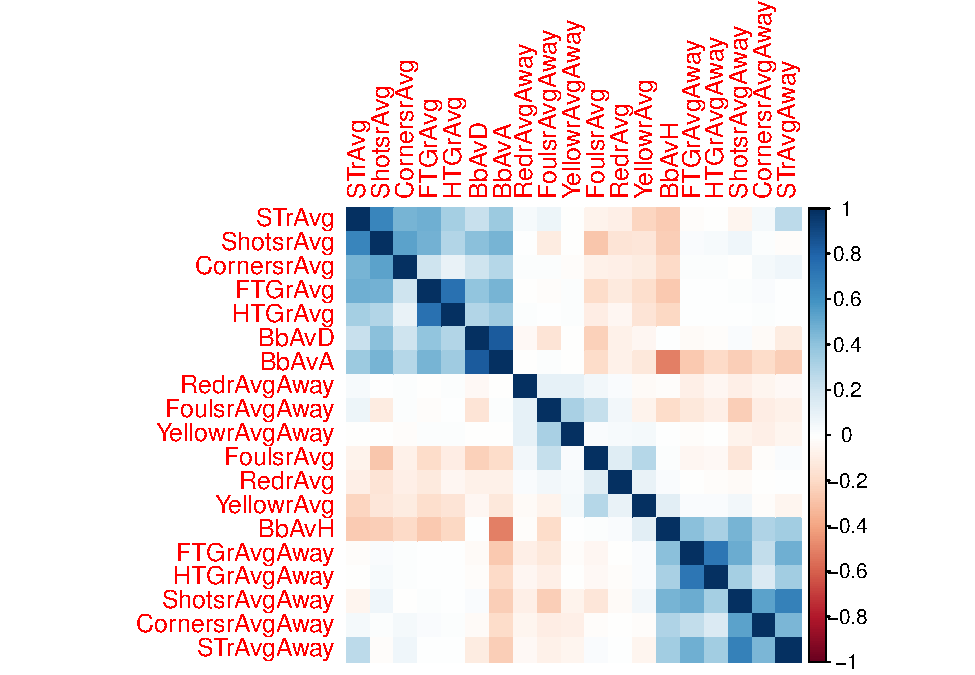
\includegraphics{EPL_Model_files/figure-latex/unnamed-chunk-5-1} \end{center}

The histogram mosaic below shows the distribution of the various
variables. Because the variables are all of different units, It is
important to standardize (normalize) it, hence the variables with the
highest variance dominate the PCA Analysis. I will be excluding the Red
cards due to how unfrequent they are. I will log transform the betting
avergaes to get the data as close to normal as possible.

\begin{Shaded}
\begin{Highlighting}[]
\NormalTok{ModelData[,}\DecValTok{2}\OperatorTok{:}\KeywordTok{ncol}\NormalTok{(ModelData)]}\OperatorTok\KeywordTok{gather}\NormalTok{()}\OperatorTok\KeywordTok{ggplot}\NormalTok{(}\KeywordTok{aes}\NormalTok{(value))}\OperatorTok{+}\KeywordTok{facet_wrap}\NormalTok{(}\OperatorTok{~}\NormalTok{key, }\DataTypeTok{scales =} \StringTok{"free"}\NormalTok{)}\OperatorTok{+}\KeywordTok{geom_histogram}\NormalTok{()}
\end{Highlighting}
\end{Shaded}

\begin{verbatim}
## `stat_bin()` using `bins = 30`. Pick better value with `binwidth`.
\end{verbatim}

\begin{center}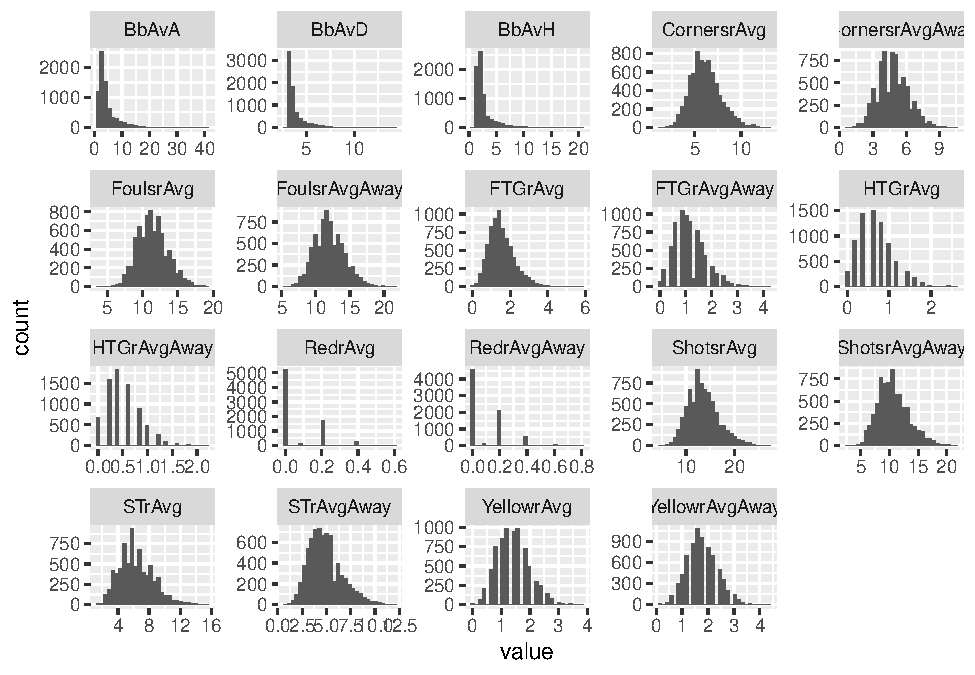
\includegraphics{EPL_Model_files/figure-latex/unnamed-chunk-6-1} \end{center}

\begin{Shaded}
\begin{Highlighting}[]
\CommentTok{#transform model data}
\NormalTok{ModelData[,}\StringTok{`}\DataTypeTok{:=}\StringTok{`}\NormalTok{ (}\DataTypeTok{BbAvA=}\KeywordTok{log}\NormalTok{(BbAvA), }\DataTypeTok{BbAvD=}\KeywordTok{log}\NormalTok{(BbAvD), }\DataTypeTok{BbAvH=}\KeywordTok{log}\NormalTok{(BbAvH), }\DataTypeTok{FTR=} \KeywordTok{as.factor}\NormalTok{(FTR))]}
\NormalTok{ModelData[,}\StringTok{`}\DataTypeTok{:=}\StringTok{`}\NormalTok{ (}\DataTypeTok{RedrAvg =} \OtherTok{NULL}\NormalTok{, }\DataTypeTok{RedrAvgAway =} \OtherTok{NULL}\NormalTok{)]}
\NormalTok{ModelData[,}\DecValTok{2}\OperatorTok{:}\KeywordTok{ncol}\NormalTok{(ModelData)]}\OperatorTok\KeywordTok{gather}\NormalTok{()}\OperatorTok\KeywordTok{ggplot}\NormalTok{(}\KeywordTok{aes}\NormalTok{(value))}\OperatorTok{+}\KeywordTok{facet_wrap}\NormalTok{(}\OperatorTok{~}\NormalTok{key, }\DataTypeTok{scales =} \StringTok{"free"}\NormalTok{)}\OperatorTok{+}\KeywordTok{geom_histogram}\NormalTok{()}
\end{Highlighting}
\end{Shaded}

\begin{verbatim}
## `stat_bin()` using `bins = 30`. Pick better value with `binwidth`.
\end{verbatim}

\begin{center}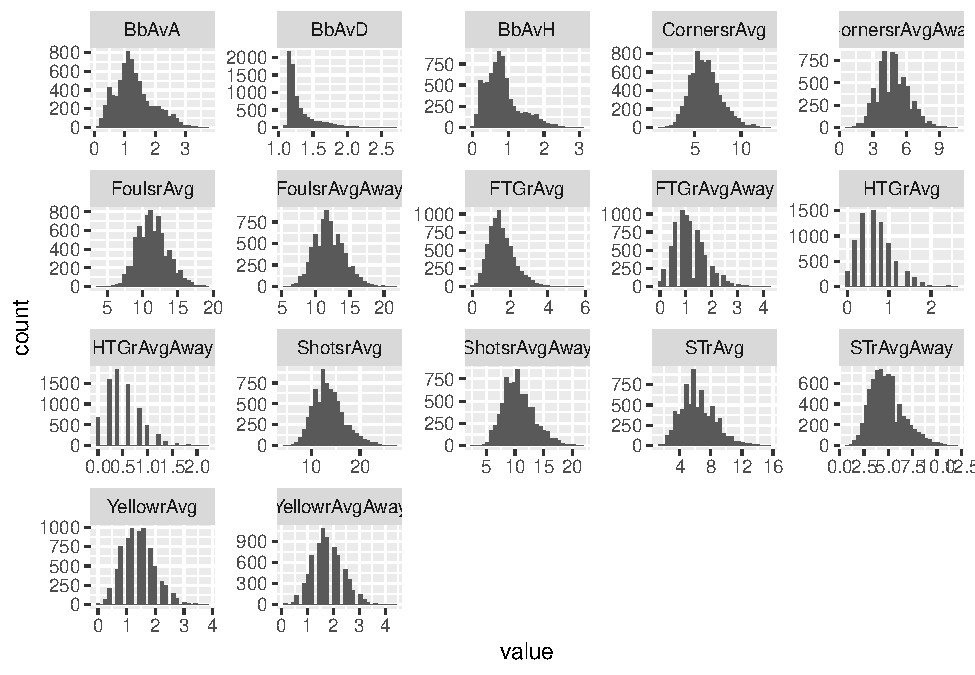
\includegraphics{EPL_Model_files/figure-latex/unnamed-chunk-6-2} \end{center}

\hypertarget{principal-component-analysis}{%
\subsection{Principal Component
Analysis}\label{principal-component-analysis}}

\begin{Shaded}
\begin{Highlighting}[]
\NormalTok{pcaEPL =}\StringTok{ }\KeywordTok{prcomp}\NormalTok{(ModelData[,}\OperatorTok{-}\DecValTok{1}\NormalTok{], }\DataTypeTok{scale=}\NormalTok{T)}
\KeywordTok{fviz_eig}\NormalTok{(pcaEPL, }\DataTypeTok{addlabels =}\NormalTok{ T)}
\end{Highlighting}
\end{Shaded}

\begin{center}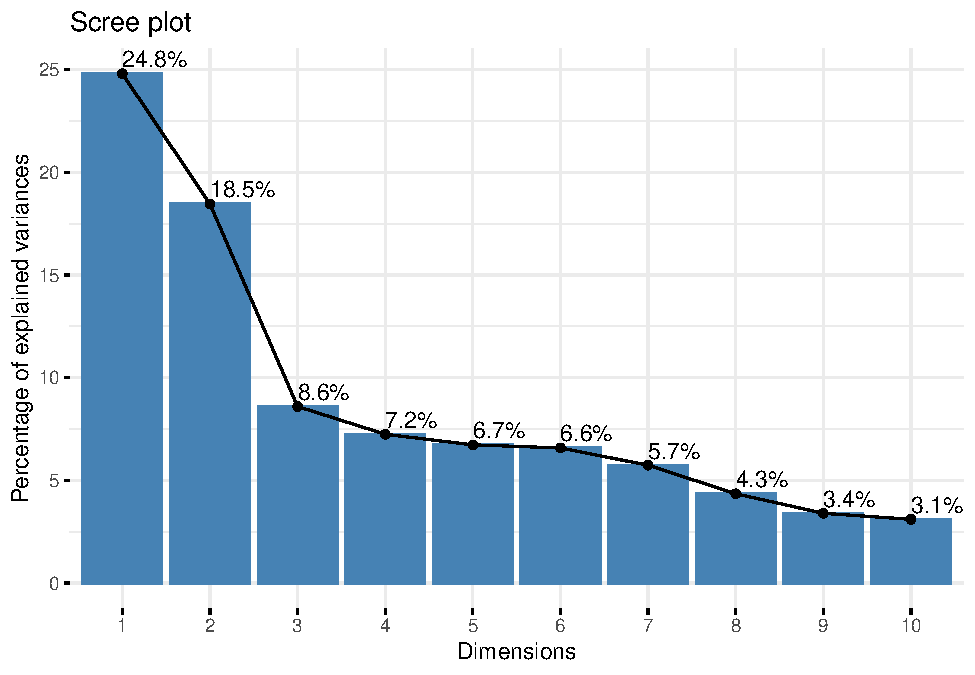
\includegraphics{EPL_Model_files/figure-latex/unnamed-chunk-7-1} \end{center}

\begin{Shaded}
\begin{Highlighting}[]
\CommentTok{#summary(pcaEPL)}
\CommentTok{#Variables}
\KeywordTok{fviz_pca_var}\NormalTok{(pcaEPL,}
             \DataTypeTok{col.var =} \StringTok{"contrib"}\NormalTok{, }\CommentTok{# Color by contributions to the PC}
             \DataTypeTok{gradient.cols =} \KeywordTok{c}\NormalTok{(}\StringTok{"#00AFBB"}\NormalTok{, }\StringTok{"#E7B800"}\NormalTok{, }\StringTok{"#FC4E07"}\NormalTok{),}
             \DataTypeTok{repel =} \OtherTok{TRUE}     \CommentTok{# Avoid text overlapping}
\NormalTok{             )}
\end{Highlighting}
\end{Shaded}

\begin{center}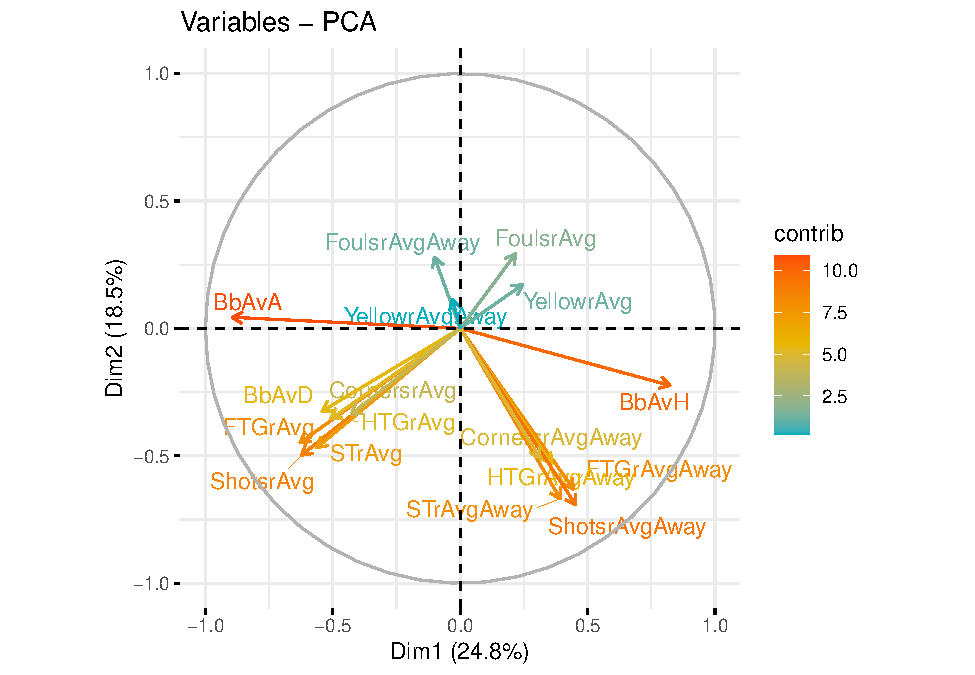
\includegraphics{EPL_Model_files/figure-latex/unnamed-chunk-7-2} \end{center}

\begin{Shaded}
\begin{Highlighting}[]
\CommentTok{#PCA result}
\NormalTok{eplVariablesPCA =}\StringTok{ }\KeywordTok{get_pca_var}\NormalTok{(pcaEPL)}
\CommentTok{#eplVariablesPCA$coord}
\CommentTok{#eplVariablesPCA$contrib}

\NormalTok{variableContribbution =}\StringTok{ }\KeywordTok{as.data.frame}\NormalTok{(}\KeywordTok{sort}\NormalTok{(}\KeywordTok{rowSums}\NormalTok{(eplVariablesPCA}\OperatorTok{$}\NormalTok{contrib[,}\DecValTok{1}\OperatorTok{:}\DecValTok{2}\NormalTok{])))}
\KeywordTok{names}\NormalTok{(variableContribbution) =}\StringTok{ }\KeywordTok{c}\NormalTok{(}\StringTok{"PCA_Contribution"}\NormalTok{)}
\KeywordTok{ggplot}\NormalTok{(variableContribbution, }\KeywordTok{aes}\NormalTok{(}\DataTypeTok{x =} \KeywordTok{row.names}\NormalTok{(variableContribbution), }\DataTypeTok{y =}\NormalTok{ PCA_Contribution))}\OperatorTok{+}\StringTok{ }\KeywordTok{geom_bar}\NormalTok{(}\DataTypeTok{stat =} \StringTok{"identity"}\NormalTok{, }\DataTypeTok{fill=}\StringTok{"steelblue"}\NormalTok{)}\OperatorTok{+}\StringTok{ }
\StringTok{  }\KeywordTok{theme}\NormalTok{(}\DataTypeTok{axis.text.x=}\KeywordTok{element_text}\NormalTok{(}\DataTypeTok{angle=}\DecValTok{90}\NormalTok{, }\DataTypeTok{hjust =} \DecValTok{1}\NormalTok{))}\OperatorTok{+}\KeywordTok{xlab}\NormalTok{(}\StringTok{"PCA contribution to the first 2 dimensions"}\NormalTok{)}
\end{Highlighting}
\end{Shaded}

\begin{center}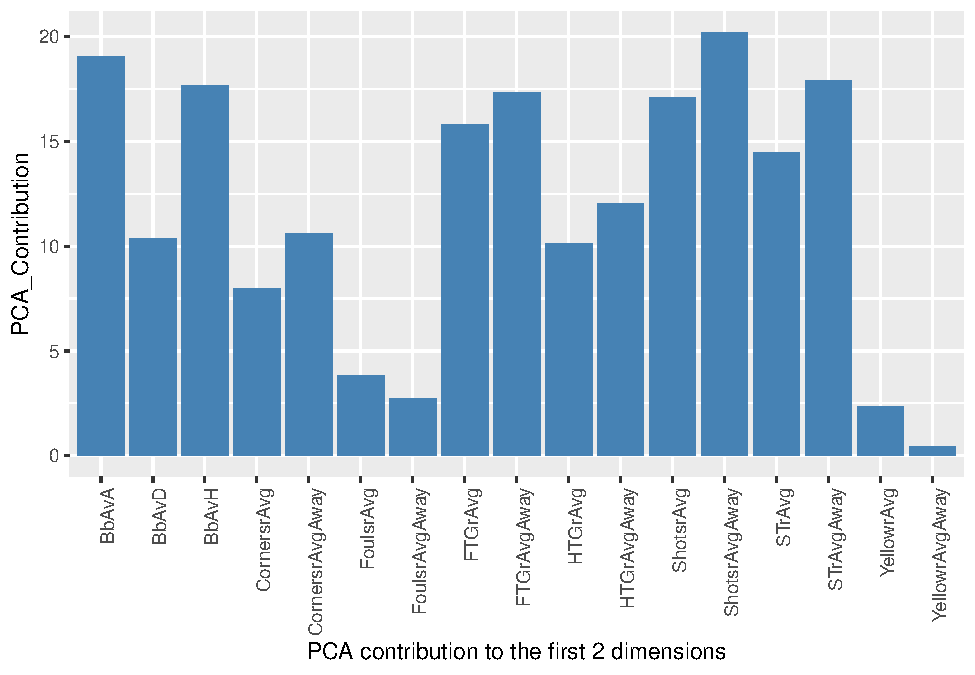
\includegraphics{EPL_Model_files/figure-latex/unnamed-chunk-7-3} \end{center}

\hypertarget{cart-tree-with-k-fold-cross-validation}{%
\subsection{CART Tree with k-Fold cross
validation}\label{cart-tree-with-k-fold-cross-validation}}

\begin{Shaded}
\begin{Highlighting}[]
\CommentTok{#Classification Tree}
\NormalTok{EPLTree <-}\StringTok{ }\KeywordTok{rpart}\NormalTok{(FTR}\OperatorTok{~}\StringTok{ }\NormalTok{.}\OperatorTok{-}\NormalTok{FoulsrAvg  }\OperatorTok{-}\NormalTok{FoulsrAvgAway }\OperatorTok{-}\NormalTok{YellowrAvg }\OperatorTok{-}\NormalTok{YellowrAvgAway , }\DataTypeTok{data=}\NormalTok{ ModelData, }\DataTypeTok{method =} \StringTok{"class"}\NormalTok{)}
\KeywordTok{fancyRpartPlot}\NormalTok{(EPLTree)}
\end{Highlighting}
\end{Shaded}

\begin{center}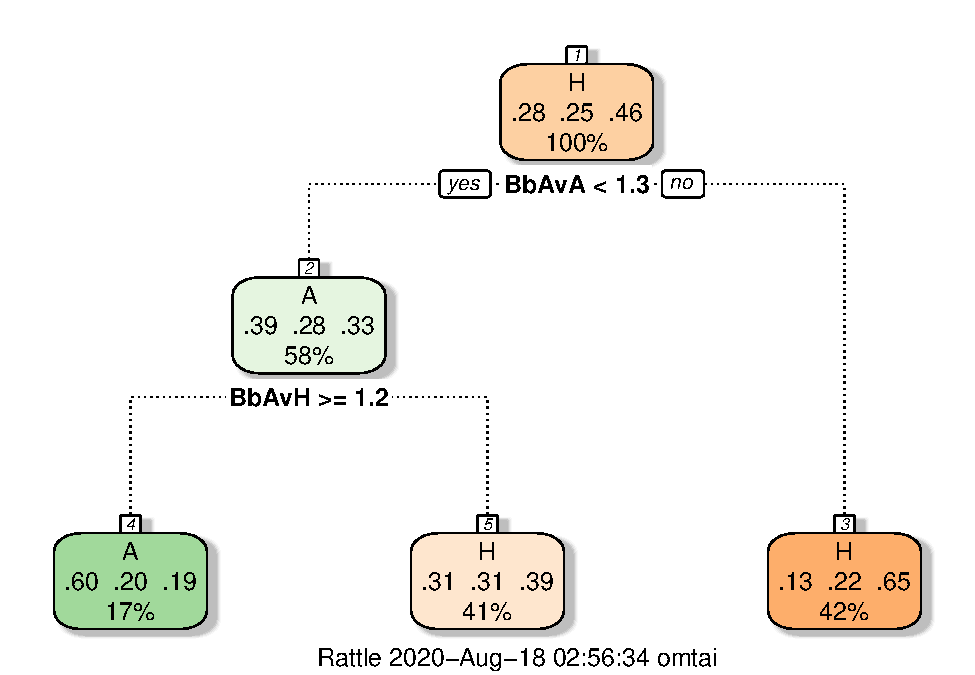
\includegraphics{EPL_Model_files/figure-latex/unnamed-chunk-8-1} \end{center}

\begin{Shaded}
\begin{Highlighting}[]
\CommentTok{#printcp(EPLTree)}
\KeywordTok{plotcp}\NormalTok{(EPLTree)}
\end{Highlighting}
\end{Shaded}

\begin{center}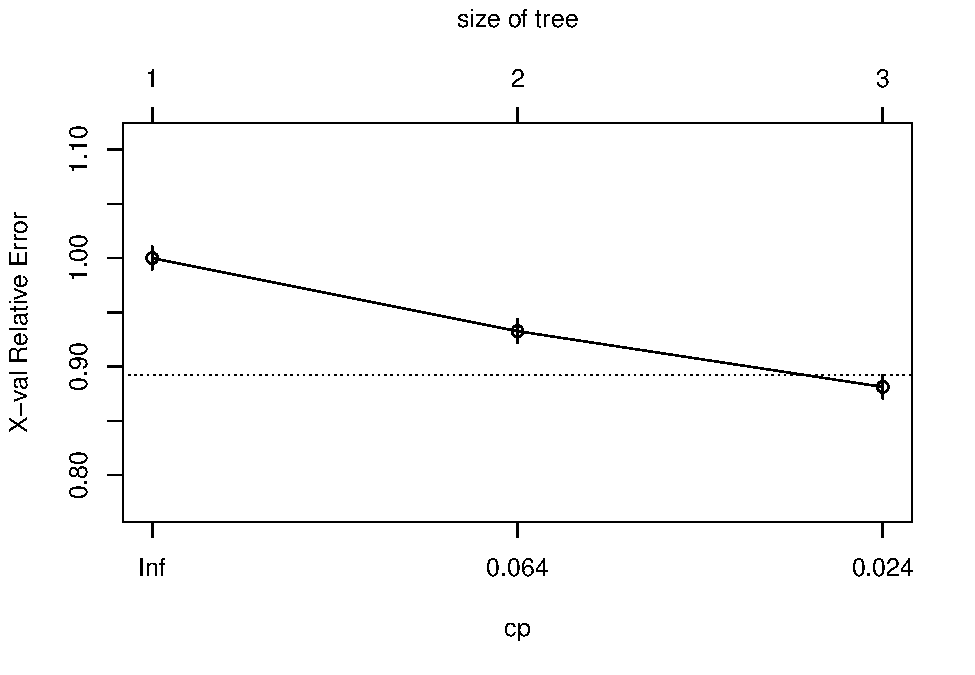
\includegraphics{EPL_Model_files/figure-latex/unnamed-chunk-8-2} \end{center}

\begin{Shaded}
\begin{Highlighting}[]
\CommentTok{#Predicion - All data}
\NormalTok{ModelData}\OperatorTok{$}\NormalTok{predictFT =}\StringTok{ }\KeywordTok{predict}\NormalTok{(EPLTree, }\DataTypeTok{type =} \StringTok{"class"}\NormalTok{)}
\NormalTok{cm <-}\StringTok{ }\KeywordTok{conf_mat}\NormalTok{(ModelData, FTR, predictFT)}
\KeywordTok{plot_confusion_matrix}\NormalTok{(cm)}
\end{Highlighting}
\end{Shaded}

\begin{verbatim}
## Scale for 'fill' is already present. Adding another scale for 'fill', which
## will replace the existing scale.
\end{verbatim}

\begin{center}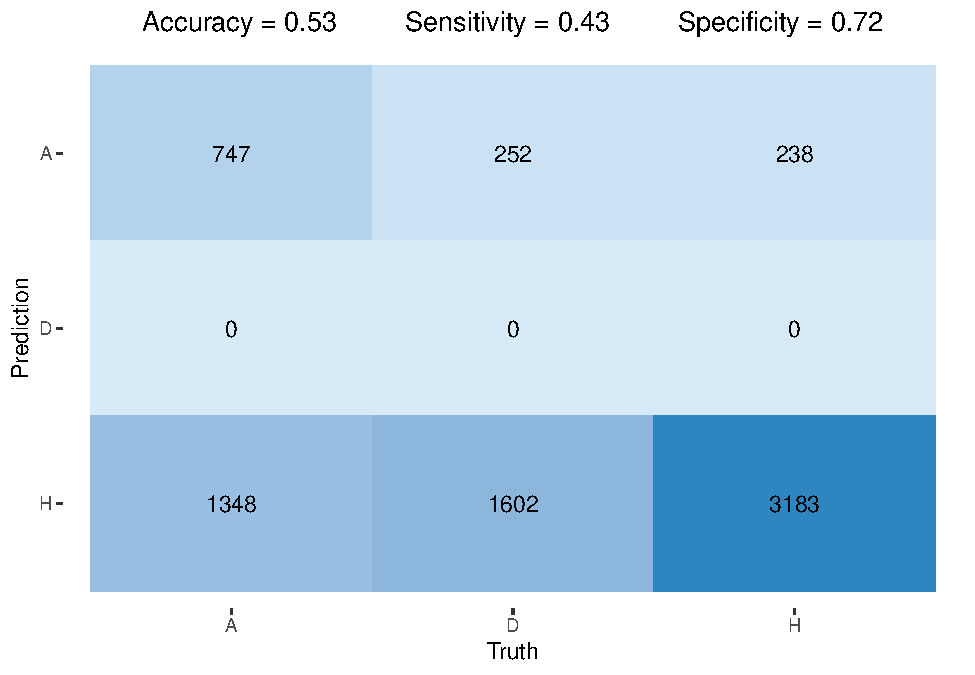
\includegraphics{EPL_Model_files/figure-latex/unnamed-chunk-8-3} \end{center}

\begin{Shaded}
\begin{Highlighting}[]
\CommentTok{#Collect Train and Test Data}
\KeywordTok{set.seed}\NormalTok{(}\DecValTok{3000}\NormalTok{)}
\NormalTok{trainIndex =}\StringTok{ }\KeywordTok{createDataPartition}\NormalTok{(ModelData}\OperatorTok{$}\NormalTok{FTR, }\DataTypeTok{p =} \FloatTok{0.7}\NormalTok{, }\DataTypeTok{list =}\NormalTok{ F, }\DataTypeTok{times =} \DecValTok{1}\NormalTok{) }
\NormalTok{Train =}\StringTok{ }\NormalTok{ModelData[trainIndex,]}
\NormalTok{Test =}\StringTok{ }\NormalTok{ModelData[}\OperatorTok{-}\NormalTok{trainIndex,]}

\CommentTok{#Cross Validation}
\NormalTok{numFolds <-}\StringTok{ }\KeywordTok{trainControl}\NormalTok{(}\DataTypeTok{method=}\StringTok{"cv"}\NormalTok{, }\DataTypeTok{number=}\DecValTok{10}\NormalTok{, }\DataTypeTok{repeats =} \DecValTok{10}\NormalTok{)}
\NormalTok{cpGrid <-}\StringTok{ }\KeywordTok{expand.grid}\NormalTok{(}\DataTypeTok{.cp=}\KeywordTok{seq}\NormalTok{(}\FloatTok{0.001}\NormalTok{,}\FloatTok{0.01}\NormalTok{,}\FloatTok{0.001}\NormalTok{))}\CommentTok{#cp paramaeters to test as numbers from 0.0005 to 0.05, in increments of 0.01.}
\NormalTok{treeTuning =}\StringTok{ }\KeywordTok{train}\NormalTok{(FTR}\OperatorTok{~}\NormalTok{.}\OperatorTok{-}\NormalTok{FoulsrAvg  }\OperatorTok{-}\NormalTok{FoulsrAvgAway }\OperatorTok{-}\NormalTok{YellowrAvg }\OperatorTok{-}\NormalTok{YellowrAvgAway, }\DataTypeTok{data =}\NormalTok{ Train, }\DataTypeTok{method=}\StringTok{"rpart"}\NormalTok{, }\DataTypeTok{trControl=}\NormalTok{numFolds, }\DataTypeTok{tuneGrid =}\NormalTok{ cpGrid) }\CommentTok{#cp = 0.0155}
\KeywordTok{plot}\NormalTok{(treeTuning)}
\end{Highlighting}
\end{Shaded}

\begin{center}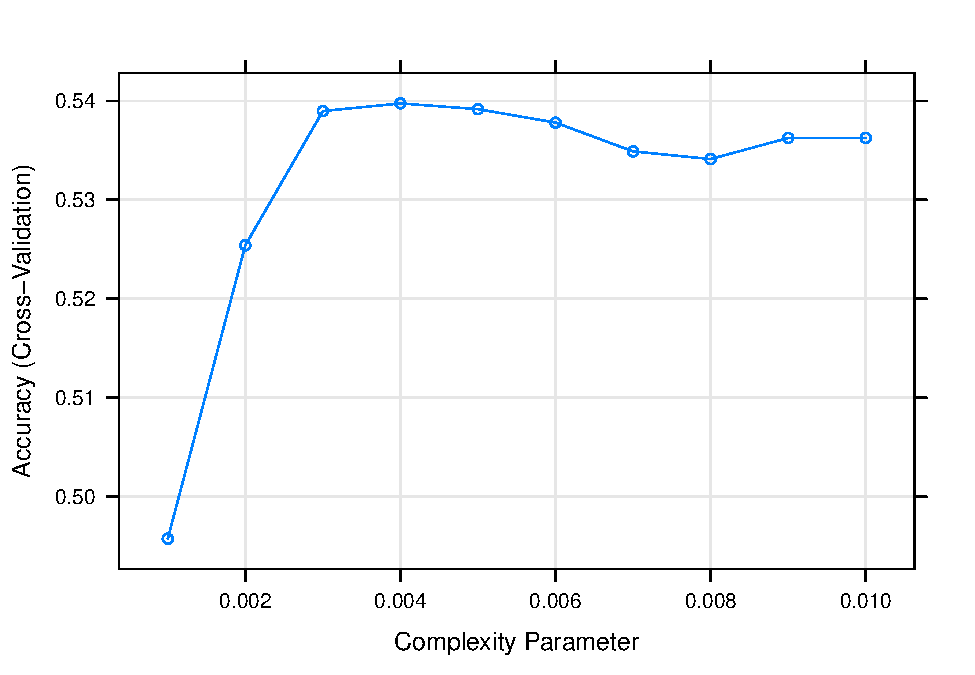
\includegraphics{EPL_Model_files/figure-latex/unnamed-chunk-8-4} \end{center}

\begin{Shaded}
\begin{Highlighting}[]
\NormalTok{treeTuning}
\end{Highlighting}
\end{Shaded}

\begin{verbatim}
## CART 
## 
## 5160 samples
##   18 predictor
##    3 classes: 'A', 'D', 'H' 
## 
## No pre-processing
## Resampling: Cross-Validated (10 fold) 
## Summary of sample sizes: 4643, 4645, 4644, 4644, 4645, 4644, ... 
## Resampling results across tuning parameters:
## 
##   cp     Accuracy   Kappa    
##   0.001  0.4957548  0.1831466
##   0.002  0.5254008  0.2082387
##   0.003  0.5389611  0.2224991
##   0.004  0.5397359  0.2221366
##   0.005  0.5391538  0.2207803
##   0.006  0.5377968  0.2180318
##   0.007  0.5348872  0.2123516
##   0.008  0.5341116  0.2143880
##   0.009  0.5362434  0.2173852
##   0.010  0.5362442  0.2164838
## 
## Accuracy was used to select the optimal model using the largest value.
## The final value used for the model was cp = 0.004.
\end{verbatim}

\begin{Shaded}
\begin{Highlighting}[]
\CommentTok{#Classification Tree - With Validation Set}
\NormalTok{EPLTree =}\StringTok{ }\KeywordTok{rpart}\NormalTok{(FTR}\OperatorTok{~}\StringTok{ }\NormalTok{.}\OperatorTok{-}\NormalTok{FoulsrAvg  }\OperatorTok{-}\NormalTok{FoulsrAvgAway }\OperatorTok{-}\NormalTok{YellowrAvg }\OperatorTok{-}\NormalTok{YellowrAvgAway, }\DataTypeTok{data=}\NormalTok{ Train, }\DataTypeTok{method =} \StringTok{"class"}\NormalTok{,  }\DataTypeTok{cp =} \FloatTok{0.004}\NormalTok{)}
\KeywordTok{fancyRpartPlot}\NormalTok{(EPLTree)}
\end{Highlighting}
\end{Shaded}

\begin{center}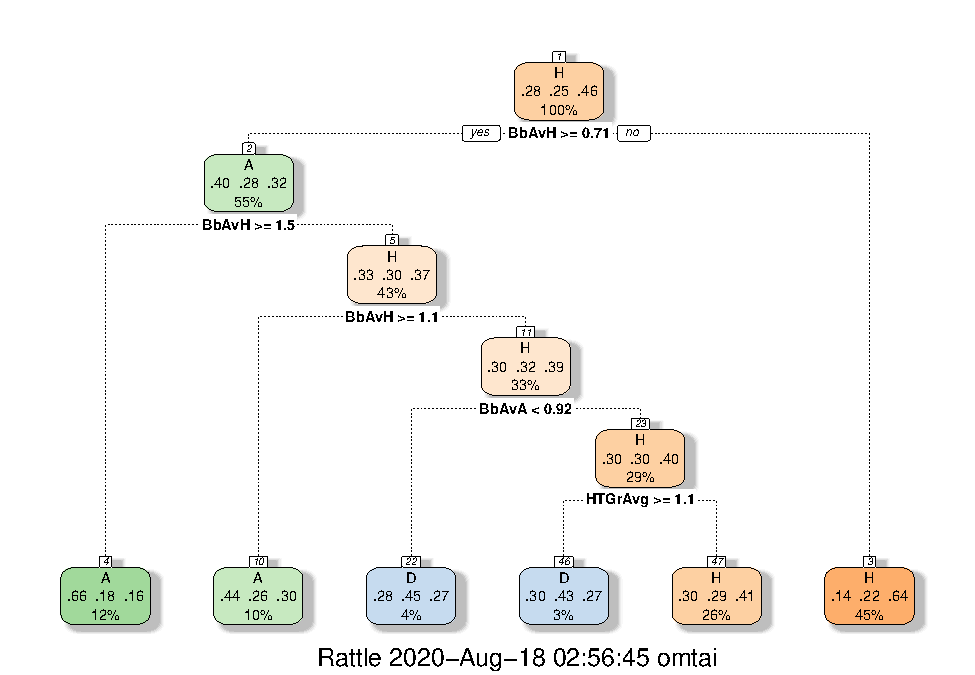
\includegraphics{EPL_Model_files/figure-latex/unnamed-chunk-8-5} \end{center}

\begin{Shaded}
\begin{Highlighting}[]
\CommentTok{#Predicion - Test data}
\NormalTok{Test}\OperatorTok{$}\NormalTok{predictFT =}\StringTok{ }\KeywordTok{predict}\NormalTok{(EPLTree, }\DataTypeTok{type =} \StringTok{"class"}\NormalTok{, }\DataTypeTok{newdata =}\NormalTok{ Test)}
\NormalTok{cm =}\StringTok{ }\KeywordTok{conf_mat}\NormalTok{(Test, FTR, predictFT)}
\KeywordTok{plot_confusion_matrix}\NormalTok{(cm)}
\end{Highlighting}
\end{Shaded}

\begin{verbatim}
## Scale for 'fill' is already present. Adding another scale for 'fill', which
## will replace the existing scale.
\end{verbatim}

\begin{center}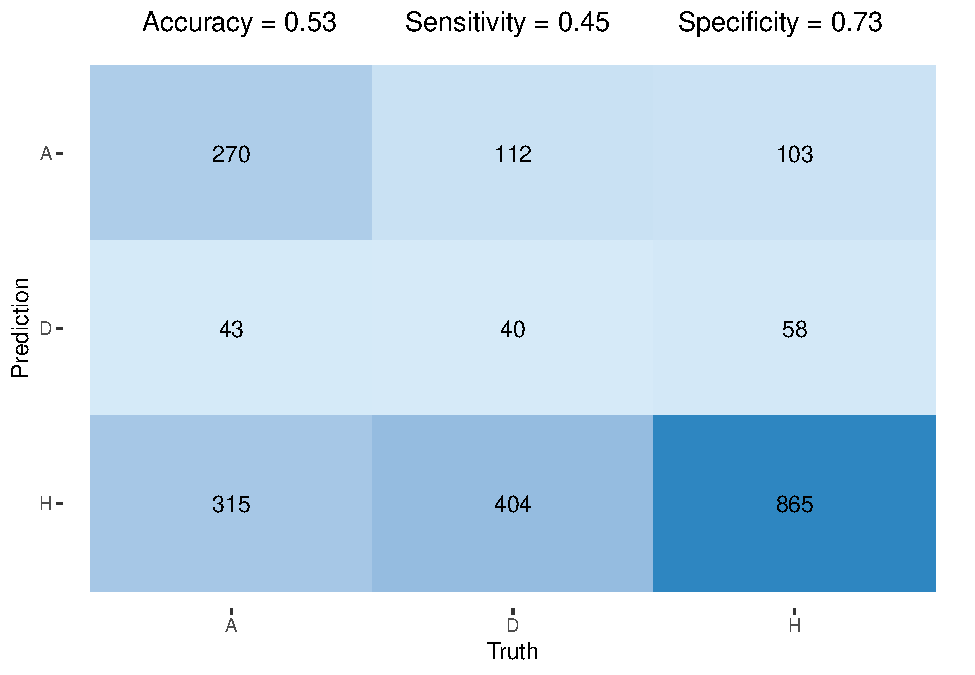
\includegraphics{EPL_Model_files/figure-latex/unnamed-chunk-8-6} \end{center}

\hypertarget{random-forest}{%
\subsection{Random Forest}\label{random-forest}}

\begin{Shaded}
\begin{Highlighting}[]
\NormalTok{EPLForest =}\StringTok{ }\KeywordTok{randomForest}\NormalTok{(FTR}\OperatorTok{~}\NormalTok{., }\DataTypeTok{data=}\NormalTok{ Train, }\DataTypeTok{mtry =}\DecValTok{4}\NormalTok{, }\DataTypeTok{ntree =} \DecValTok{1000}\NormalTok{)}
\NormalTok{Test}\OperatorTok{$}\NormalTok{predictFT =}\StringTok{ }\KeywordTok{predict}\NormalTok{(EPLForest, }\DataTypeTok{type =} \StringTok{"class"}\NormalTok{, }\DataTypeTok{newdata =}\NormalTok{ Test)}
\NormalTok{cm <-}\StringTok{ }\KeywordTok{conf_mat}\NormalTok{(Test, FTR, predictFT)}
\KeywordTok{plot_confusion_matrix}\NormalTok{(cm)}
\end{Highlighting}
\end{Shaded}

\begin{verbatim}
## Scale for 'fill' is already present. Adding another scale for 'fill', which
## will replace the existing scale.
\end{verbatim}

\begin{center}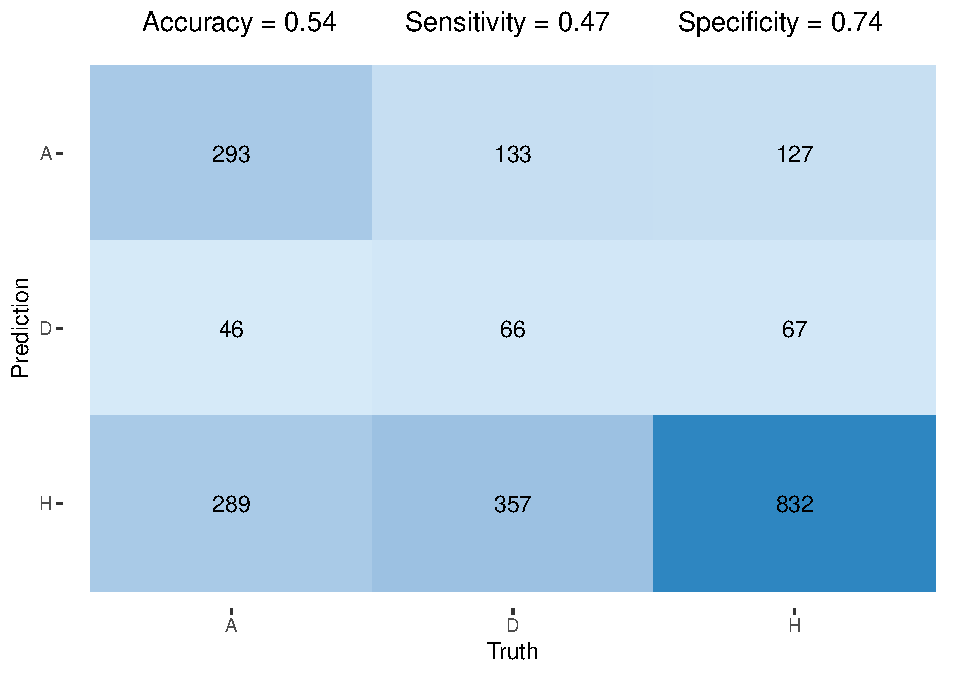
\includegraphics{EPL_Model_files/figure-latex/unnamed-chunk-9-1} \end{center}

\begin{Shaded}
\begin{Highlighting}[]
\CommentTok{# Tune Parameters}
\CommentTok{# control = trainControl(method="repeatedcv", number=10, repeats=3, search="grid")}
\CommentTok{# tunegrid = expand.grid(.mtry =c(1:5))}
\CommentTok{# rfGrid <- train(FTR~., data=Train, method="rf", metric="Accuracy", tuneGrid=tunegrid, trControl = control, ntree = 500)}
\CommentTok{# print(rfGrid)}
\CommentTok{# plot(rfGrid)}
\end{Highlighting}
\end{Shaded}

\hypertarget{multinomial-logistic-regression}{%
\subsection{Multinomial Logistic
Regression}\label{multinomial-logistic-regression}}

\begin{Shaded}
\begin{Highlighting}[]
\NormalTok{glmModel =}\StringTok{ }\KeywordTok{multinom}\NormalTok{(FTR}\OperatorTok{~}\NormalTok{.}\OperatorTok{-}\NormalTok{FoulsrAvg  }\OperatorTok{-}\NormalTok{FoulsrAvgAway }\OperatorTok{-}\NormalTok{YellowrAvg }\OperatorTok{-}\NormalTok{YellowrAvgAway, }\DataTypeTok{data=}\NormalTok{ Train)}
\end{Highlighting}
\end{Shaded}

\begin{verbatim}
## # weights:  51 (32 variable)
## initial  value 5668.839410 
## iter  10 value 5169.756715
## iter  20 value 5026.583400
## iter  30 value 4952.566469
## final  value 4949.762794 
## converged
\end{verbatim}

\begin{Shaded}
\begin{Highlighting}[]
\CommentTok{#summary(glmModel)}
\NormalTok{Test}\OperatorTok{$}\NormalTok{predictFT =}\StringTok{ }\KeywordTok{predict}\NormalTok{(glmModel,Test, }\StringTok{"class"}\NormalTok{)}
\NormalTok{cm <-}\StringTok{ }\KeywordTok{conf_mat}\NormalTok{(Test, FTR, predictFT)}
\KeywordTok{plot_confusion_matrix}\NormalTok{(cm)}
\end{Highlighting}
\end{Shaded}

\begin{verbatim}
## Scale for 'fill' is already present. Adding another scale for 'fill', which
## will replace the existing scale.
\end{verbatim}

\begin{center}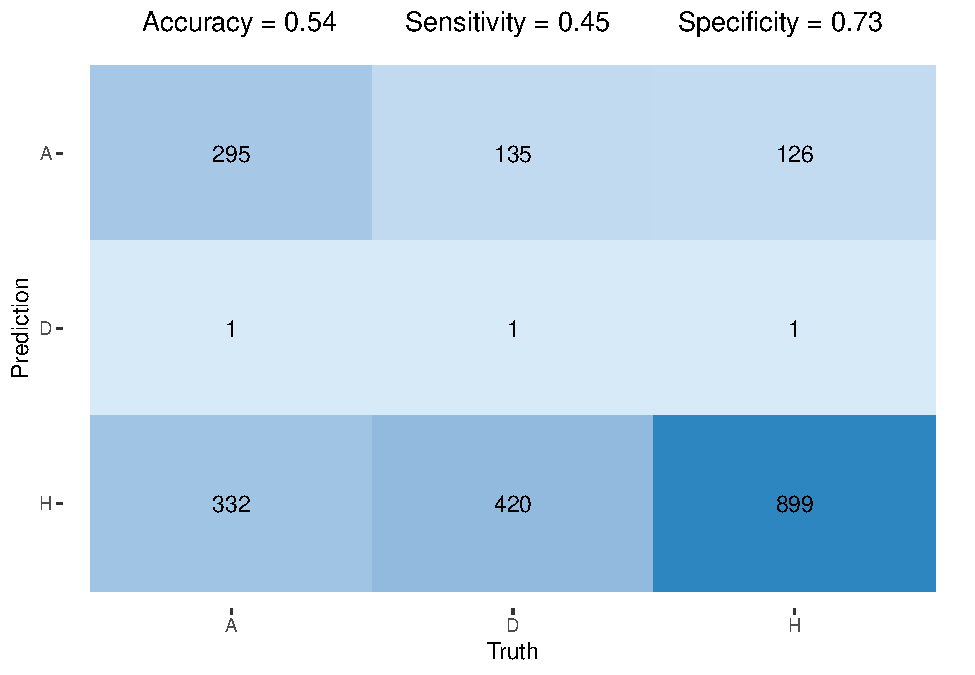
\includegraphics{EPL_Model_files/figure-latex/unnamed-chunk-10-1} \end{center}

\hypertarget{linear-discriminant-analysis-and-quadratic-discriminat-analysis}{%
\subsection{Linear Discriminant Analysis and Quadratic Discriminat
Analysis}\label{linear-discriminant-analysis-and-quadratic-discriminat-analysis}}

\begin{Shaded}
\begin{Highlighting}[]
\CommentTok{#Log transform BbAvH for lda to normalize}
\NormalTok{ldaTrain =}\StringTok{ }\KeywordTok{copy}\NormalTok{(Train)}
\CommentTok{#ldaTrain[,BbAvH:=log(BbAvH)]}
\CommentTok{#ldaTrain[,BbAvD:=log(BbAvD)]}

\NormalTok{ldaTest =}\StringTok{ }\KeywordTok{copy}\NormalTok{(Test)}
\CommentTok{#ldaTest[,BbAvH:=log(BbAvH)]}
\CommentTok{#ldaTest[,BbAvD:=log(BbAvD)]}
\CommentTok{#ldaData = rbind(ldaTest,ldaTrain)}

\NormalTok{ldaModel =}\StringTok{ }\KeywordTok{lda}\NormalTok{(FTR}\OperatorTok{~}\NormalTok{BbAvH}\OperatorTok{+}\NormalTok{BbAvA}\OperatorTok{+}\NormalTok{BbAvD}\OperatorTok{+}\NormalTok{FTGrAvg}\OperatorTok{+}\NormalTok{STrAvg}\OperatorTok{+}\NormalTok{CornersrAvg}\OperatorTok{+}\NormalTok{FTGrAvgAway}\OperatorTok{+}\NormalTok{STrAvgAway}\OperatorTok{+}\NormalTok{CornersrAvgAway, }\DataTypeTok{data =}\NormalTok{ ldaTrain)}
\KeywordTok{library}\NormalTok{(nnet)}
\NormalTok{ldaFT =}\StringTok{ }\KeywordTok{predict}\NormalTok{(ldaModel, ldaTest)}
\NormalTok{ldaTest}\OperatorTok{$}\NormalTok{predictFT =}\StringTok{ }\NormalTok{ldaFT}\OperatorTok{$}\NormalTok{class}
\NormalTok{cm <-}\StringTok{ }\KeywordTok{conf_mat}\NormalTok{(ldaTest, FTR, predictFT)}
\KeywordTok{plot_confusion_matrix}\NormalTok{(cm)}
\end{Highlighting}
\end{Shaded}

\begin{verbatim}
## Scale for 'fill' is already present. Adding another scale for 'fill', which
## will replace the existing scale.
\end{verbatim}

\begin{center}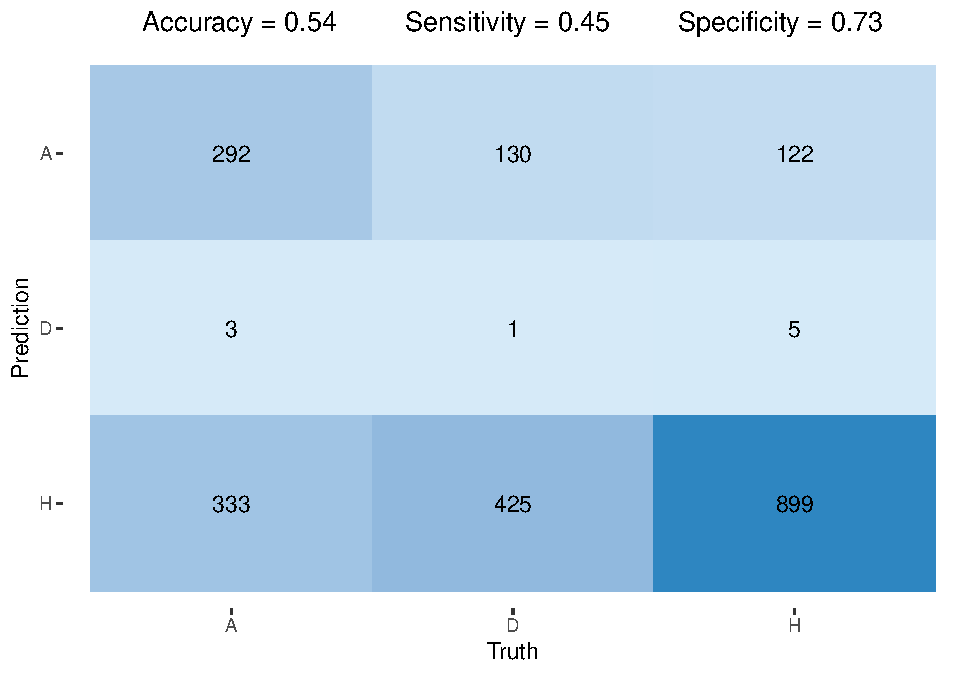
\includegraphics{EPL_Model_files/figure-latex/unnamed-chunk-11-1} \end{center}

\begin{Shaded}
\begin{Highlighting}[]
\NormalTok{qdaModel =}\StringTok{ }\KeywordTok{qda}\NormalTok{(FTR}\OperatorTok{~}\NormalTok{BbAvH}\OperatorTok{+}\NormalTok{FTGrAvg}\OperatorTok{+}\NormalTok{STrAvg}\OperatorTok{+}\NormalTok{CornersrAvg}\OperatorTok{+}\NormalTok{FTGrAvgAway}\OperatorTok{+}\NormalTok{STrAvgAway}\OperatorTok{+}\NormalTok{CornersrAvgAway, }\DataTypeTok{data =}\NormalTok{ ldaTrain)}
\NormalTok{qdaFT =}\StringTok{ }\KeywordTok{predict}\NormalTok{(qdaModel, ldaTest)}
\NormalTok{ldaTest}\OperatorTok{$}\NormalTok{predictFT =}\StringTok{ }\NormalTok{qdaFT}\OperatorTok{$}\NormalTok{class}
\NormalTok{cm <-}\StringTok{ }\KeywordTok{conf_mat}\NormalTok{(ldaTest, FTR, predictFT)}
\KeywordTok{plot_confusion_matrix}\NormalTok{(cm)}
\end{Highlighting}
\end{Shaded}

\begin{verbatim}
## Scale for 'fill' is already present. Adding another scale for 'fill', which
## will replace the existing scale.
\end{verbatim}

\begin{center}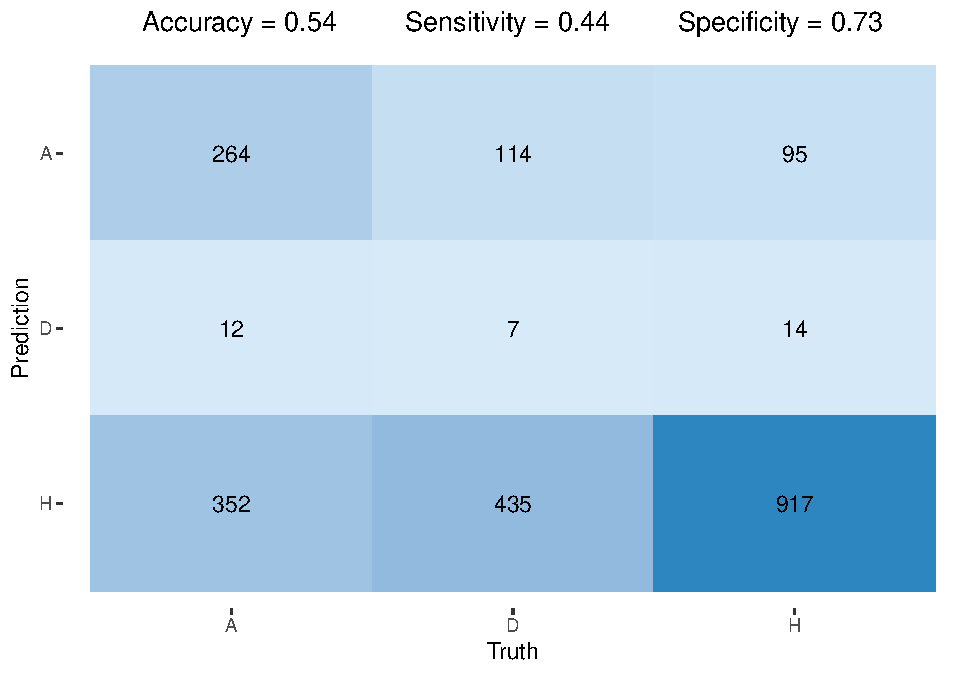
\includegraphics{EPL_Model_files/figure-latex/unnamed-chunk-11-2} \end{center}

\hypertarget{naive-bayes-classifier}{%
\subsection{Naive Bayes Classifier}\label{naive-bayes-classifier}}

\begin{Shaded}
\begin{Highlighting}[]
\NormalTok{naiveModel =}\StringTok{ }\KeywordTok{naiveBayes}\NormalTok{(FTR}\OperatorTok{~}\NormalTok{BbAvH}\OperatorTok{+}\NormalTok{FTGrAvg}\OperatorTok{+}\NormalTok{STrAvg}\OperatorTok{+}\NormalTok{CornersrAvg}\OperatorTok{+}\NormalTok{FTGrAvgAway}\OperatorTok{+}\NormalTok{STrAvgAway}\OperatorTok{+}\NormalTok{CornersrAvgAway, }\DataTypeTok{data =}\NormalTok{ ldaTrain)}
\NormalTok{ldaTest}\OperatorTok{$}\NormalTok{predictFT =}\StringTok{ }\KeywordTok{predict}\NormalTok{(naiveModel, }\DataTypeTok{type =} \StringTok{"class"}\NormalTok{, }\DataTypeTok{newdata =}\NormalTok{ ldaTest)}
\NormalTok{cm <-}\StringTok{ }\KeywordTok{conf_mat}\NormalTok{(ldaTest, FTR, predictFT)}
\KeywordTok{plot_confusion_matrix}\NormalTok{(cm)}
\end{Highlighting}
\end{Shaded}

\begin{verbatim}
## Scale for 'fill' is already present. Adding another scale for 'fill', which
## will replace the existing scale.
\end{verbatim}

\begin{center}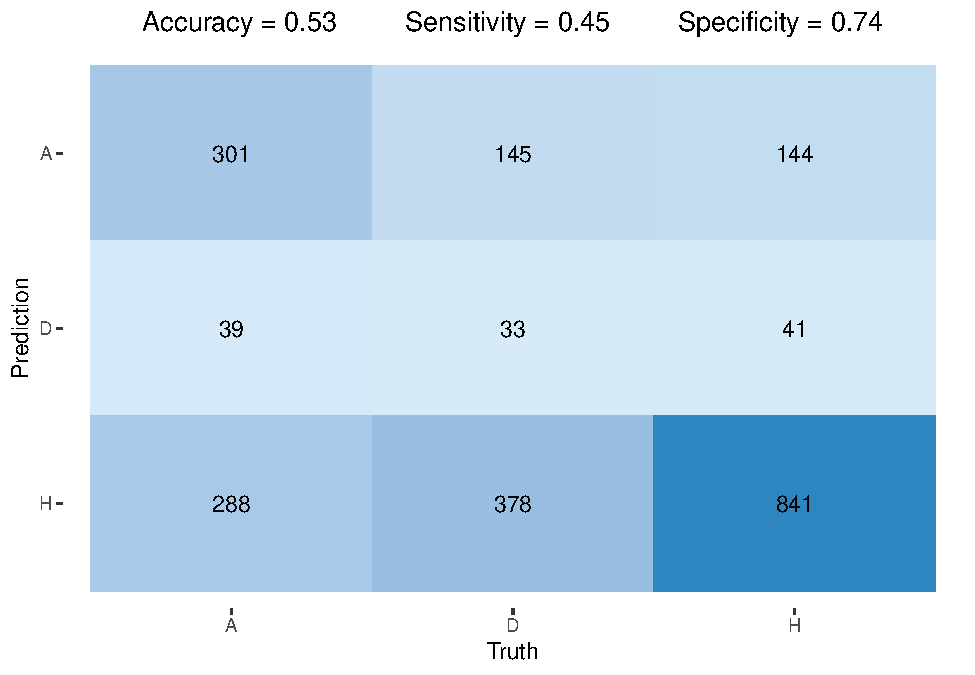
\includegraphics{EPL_Model_files/figure-latex/unnamed-chunk-12-1} \end{center}

\hypertarget{conclusion}{%
\subsection{Conclusion}\label{conclusion}}

After trying various models for prediction, I couldn't do better than a
54\% out of sample prediction accuracy. The betting odds dominate the
models as expected, due to the fact that the complex algorithms used by
the multi-billion dollar gambling industry already accounts for team
performance metrics. In the future, I plan to incorporate other
variables into my models like, team standings from previous seasons,
transfer activity in net spending, number of team injuries at time of
match, etc.

The easiest part of this was programming the models, The most
challenging aspect of the project was the data preparation, and the
other metrics I plan to include in the future will be even more
challenging due to the data coming from several different sources.

\end{document}
